\documentclass{beamer}

\usetheme{Antibes}
%\usetheme{split}
% this is a template for slides using beamer package
% adapted from slides written by Ramon Medrado
% first version: Ana Bazzan
\usecolortheme[RGB={120,0,0}]{structure}
\setbeamertemplate{blocks}[rounded][shadow=true]
\usepackage[latin1]{inputenc}
\usepackage{ragged2e}
\usepackage{graphicx}
\usepackage{caption}
\usepackage{booktabs}
\usepackage{subfig}
\usepackage{cite}

\begin{document}
\title{Work in progress}

\section{Distance matrix}
\frame{\frametitle{KITTI 00}
	\begin{center}
		\begin{figure}[ht]
			\subfloat[Distance matrix - M2DP]{%
				\includegraphics[width=0.45\textwidth]{distances_kitti00_m2dp}
			}
			~
			\subfloat[Distance matrix - CM2DP (ours)]
	\begin{center}
		\begin{figure}[ht]
			\subfloat[Distance matrix - M2DP]{%
				\includegraphics[width=0.45\textwidth]{02_distances_kitti00_m2dp}
			}
			~
			\subfloat[Distance matrix - CM2DP (ours)]{%
				\includegraphics[width=0.45\textwidth]{02_distances_kitti00_cm2dp}
			}			
			\label{fig:fig2}
		\end{figure}
	\end{center}
}

\section{Distance matrix}
\frame{\frametitle{KITTI 05}
	\begin{center}
		\begin{figure}[ht]
			\subfloat[Distance matrix - M2DP]{%
				\includegraphics[width=0.45\textwidth]{distances_kitti05_m2dp}
			}
			~
			\subfloat[Distance matrix - CM2DP (ours)]
	\begin{center}
		\begin{figure}[ht]
			\subfloat[Distance matrix - M2DP]{%
				\includegraphics[width=0.45\textwidth]{02_distances_kitti05_m2dp}
			}
			~
			\subfloat[Distance matrix - CM2DP (ours)]{%
				\includegraphics[width=0.45\textwidth]{02_distances_kitti05_cm2dp}
			}			
			\label{fig:fig4}
		\end{figure}
	\end{center}
}

\section{Distance matrix}
\frame{\frametitle{KITTI 06}
	\begin{center}
		\begin{figure}[ht]
			\subfloat[Distance matrix - M2DP]{%
				\includegraphics[width=0.45\textwidth]{distances_kitti06_m2dp}
			}
			~
			\subfloat[Distance matrix - CM2DP (ours)]
	\begin{center}
		\begin{figure}[ht]
			\subfloat[Distance matrix - M2DP]{%
				\includegraphics[width=0.45\textwidth]{02_distances_kitti06_m2dp}
			}
			~
			\subfloat[Distance matrix - CM2DP (ours)]{%
				\includegraphics[width=0.45\textwidth]{02_distances_kitti06_cm2dp}
			}			
			\label{fig:fig6}
		\end{figure}
	\end{center}
}

\section{Distance matrix}
\frame{\frametitle{KITTI 07}
	\begin{center}
		\begin{figure}[ht]
			\subfloat[Distance matrix - M2DP]{%
				\includegraphics[width=0.45\textwidth]{distances_kitti07_m2dp}
			}
			~
			\subfloat[Distance matrix - CM2DP (ours)]
	\begin{center}
		\begin{figure}[ht]
			\subfloat[Distance matrix - M2DP]{%
				\includegraphics[width=0.45\textwidth]{02_distances_kitti07_m2dp}
			}
			~
			\subfloat[Distance matrix - CM2DP (ours)]{%
				\includegraphics[width=0.45\textwidth]{02_distances_kitti07_cm2dp}
			}			
			\label{fig:fig8}
		\end{figure}
	\end{center}
}

\section{Distance matrix}
\frame{\frametitle{Freiburg 1 Room Sequence}
\begin{center}
	\begin{figure}[ht]
		\subfloat{%
			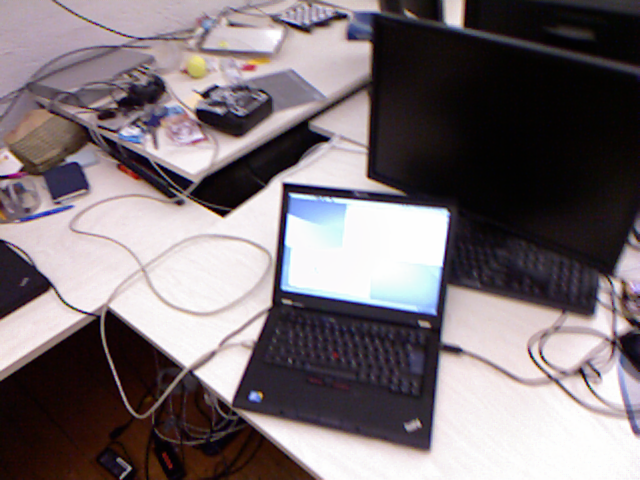
\includegraphics[width=0.30\textwidth]{fr1room1}
		}
		\subfloat{%
			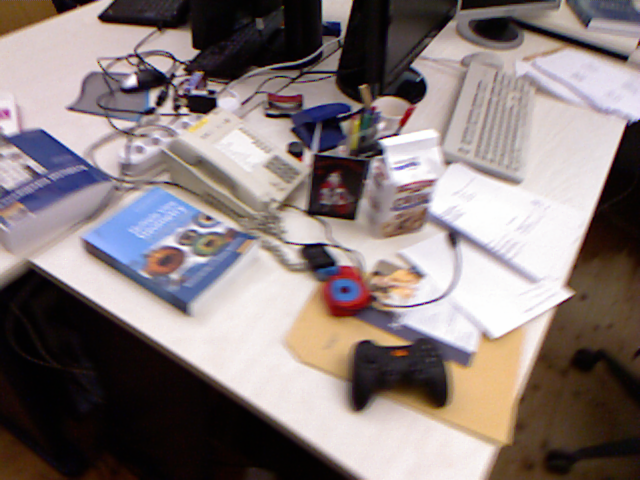
\includegraphics[width=0.30\textwidth]{fr1room2}
		}

		\subfloat{%
			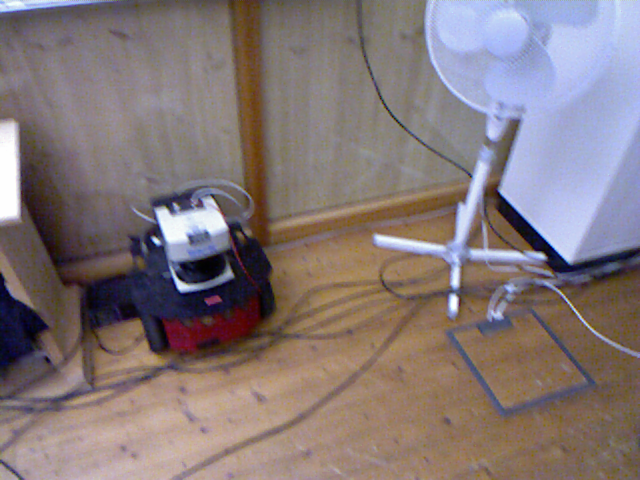
\includegraphics[width=0.30\textwidth]{fr1room3}
		}
		\subfloat{%
			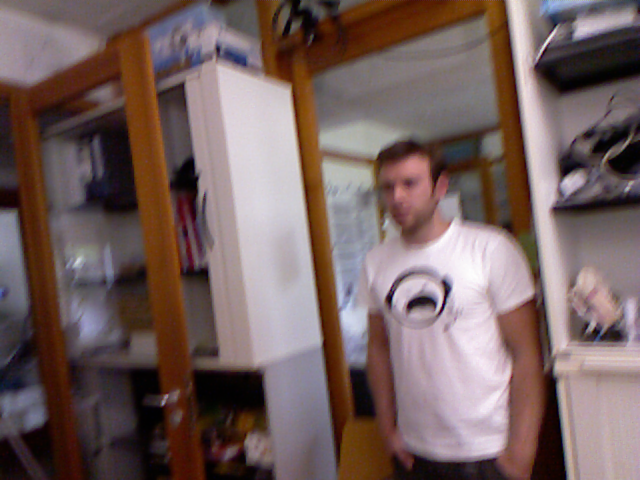
\includegraphics[width=0.30\textwidth]{fr1room4}
		}				
		\caption{Sequence samples}
		\label{fig:fig9}
	\end{figure}
\end{center}
}	

\section{Distance matrix}
\frame{\frametitle{Freiburg 1 Room Sequence}
	\begin{center}
		\begin{figure}[ht]
			\subfloat[Distance matrix - M2DP]{%
				\includegraphics[width=0.45\textwidth]{distances_fr1_room_m2dp}
			}
			~
			\subfloat[Distance matrix - CM2DP (ours)]
	\begin{center}
		\begin{figure}[ht]
			\subfloat[Distance matrix - M2DP]{%
				\includegraphics[width=0.45\textwidth]{2_distances_fr1_room_m2dp_04}
			}
			~
			\subfloat[Distance matrix - CM2DP (ours)]
	\begin{center}
		\begin{figure}[ht]
			\subfloat[Distance matrix - M2DP]{%
				\includegraphics[width=0.45\textwidth]{1_distances_fr1_room_m2dp_02}
			}
			~
			\subfloat[Distance matrix - CM2DP (ours)]{%
				\includegraphics[width=0.45\textwidth]{1_distances_fr1_room_cm2dp_02}
			}			
			\label{fig:fig12}
		\end{figure}
	\end{center}
}

\section{Distance matrix}
\frame{\frametitle{Freiburg 1 Room Sequence}
\begin{center}
	\begin{figure}[ht]
		\subfloat{%
			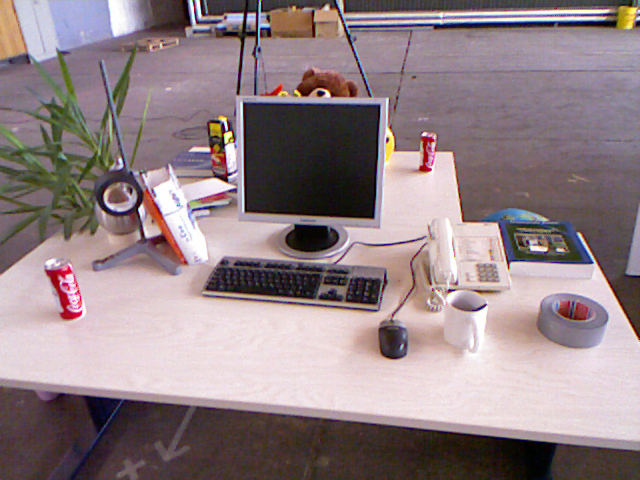
\includegraphics[width=0.30\textwidth]{fr2desk1}
		}
		\subfloat{%
			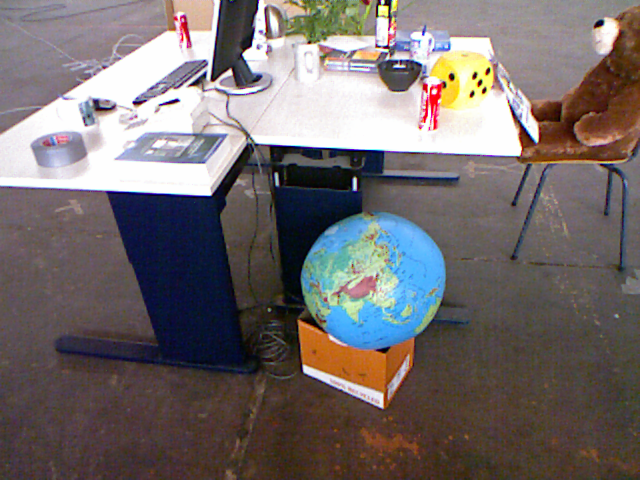
\includegraphics[width=0.30\textwidth]{fr2desk2}
		}
		
		\subfloat{%
			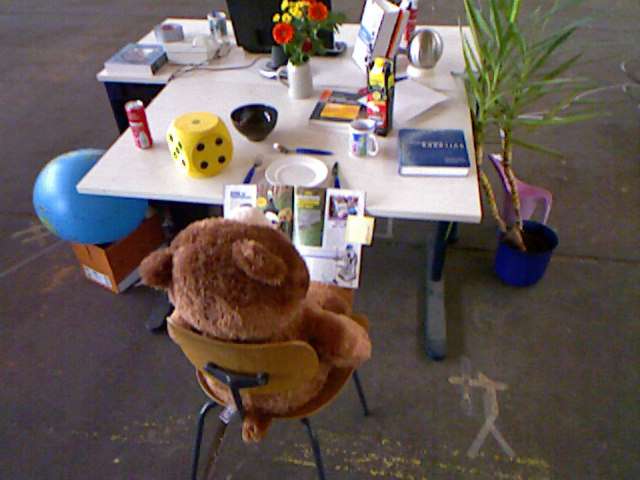
\includegraphics[width=0.30\textwidth]{fr2desk3}
		}
		\subfloat{%
			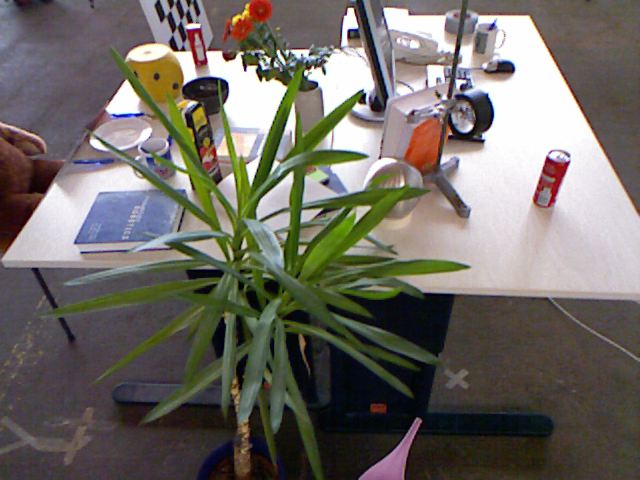
\includegraphics[width=0.30\textwidth]{fr2desk4}
		}				
		\caption{Sequence samples}
		\label{fig:fig13}
	\end{figure}
\end{center}
}		

\section{Distance matrix}
\frame{\frametitle{Freiburg 2 Desk Sequence}
	\begin{center}
		\begin{figure}[ht]
			\subfloat[Distance matrix - M2DP]{%
				\includegraphics[width=0.45\textwidth]{distances_fr2_desk_m2dp}
			}
			~
			\subfloat[Distance matrix - CM2DP (ours)]{%
				\includegraphics[width=0.45\textwidth]{distances_fr2_desk_cm2dp}
			}			
			\label{fig:fig14}
		\end{figure}
	\end{center}
}

\section{Distance matrix}
\frame{\frametitle{Freiburg 3 No Structure, Texture, Near Sequence}
	\begin{center}
		\begin{figure}[ht]
			\subfloat{%
				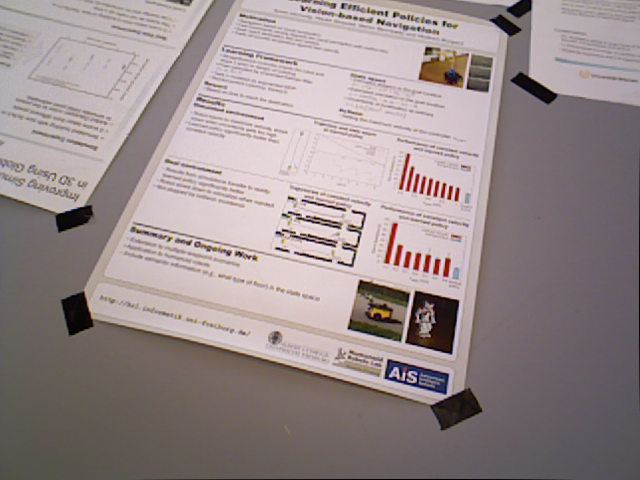
\includegraphics[width=0.30\textwidth]{fr3nostructuretexturenear1}
			}
			\subfloat{%
				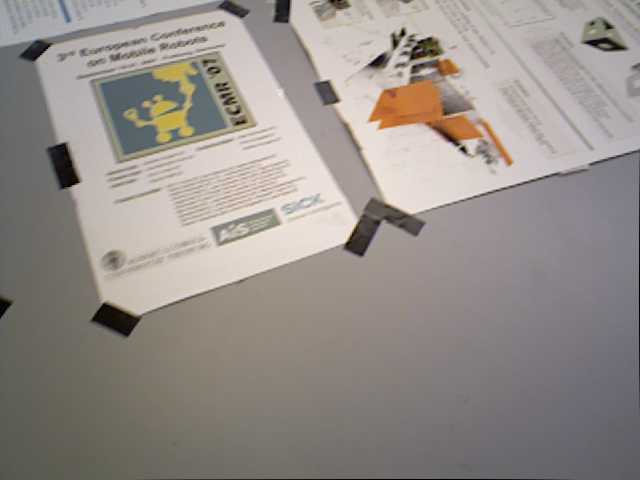
\includegraphics[width=0.30\textwidth]{fr3nostructuretexturenear2}
			}
			
			\subfloat{%
				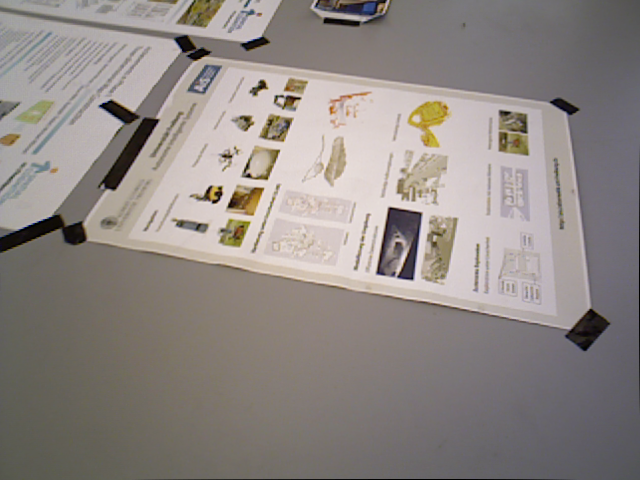
\includegraphics[width=0.30\textwidth]{fr3nostructuretexturenear3}
			}
			\subfloat{%
				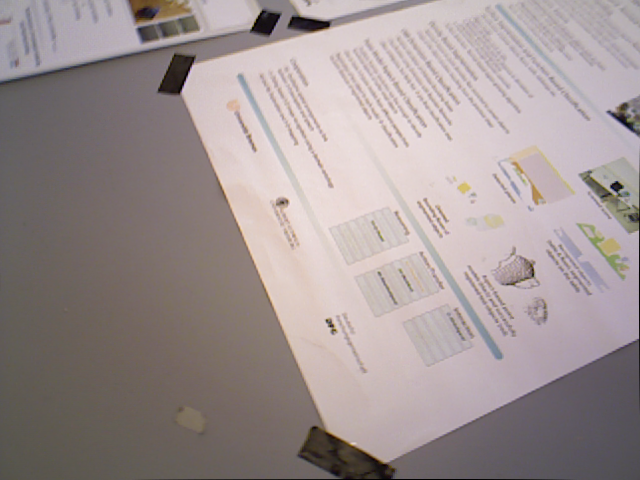
\includegraphics[width=0.30\textwidth]{fr3nostructuretexturenear4}
			}				
			\caption{Sequence samples}
			\label{fig:fig15}
		\end{figure}
	\end{center}
}		

\section{Distance matrix}
\frame{\frametitle{Freiburg 3 No Structure, Texture, Near Sequence}
	\begin{center}
		\begin{figure}[ht]
			\subfloat[Distance matrix - M2DP]{%
				\includegraphics[width=0.45\textwidth]{distances_fr3_nostructure_texture_near_withloop_m2dp}
			}
			~
			\subfloat[Distance matrix - CM2DP (ours)]{%
				\includegraphics[width=0.45\textwidth]{distances_fr3_nostructure_texture_near_withloop_cm2dp}
			}			
			\label{fig:fig16}
		\end{figure}
	\end{center}
}


\section{Distance matrix}
\frame{\frametitle{Freiburg 2 Pioneer Slam}
	\begin{center}
		\begin{figure}[ht]
			\subfloat{%
				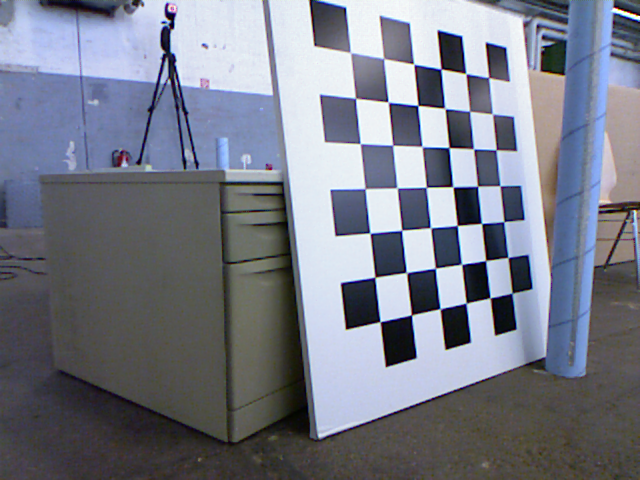
\includegraphics[width=0.30\textwidth]{fr2pioneerslam1}
			}
			\subfloat{%
				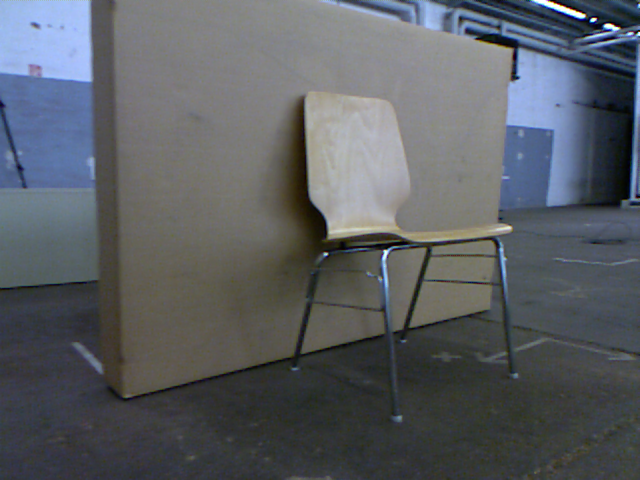
\includegraphics[width=0.30\textwidth]{fr2pioneerslam4}
			}
			
			\subfloat{%
				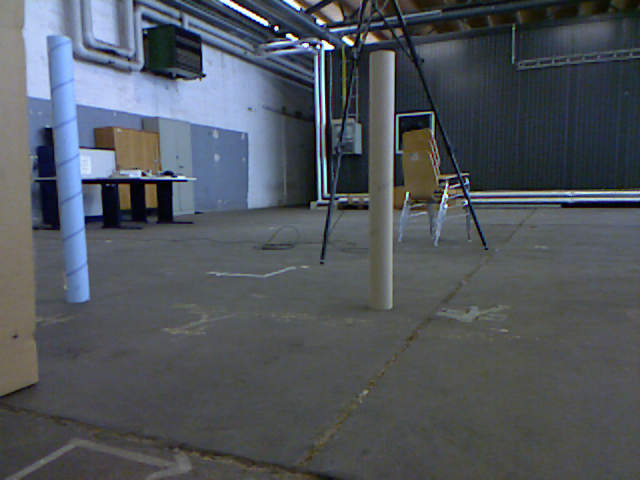
\includegraphics[width=0.30\textwidth]{fr2pioneerslam2}
			}
			\subfloat{%
				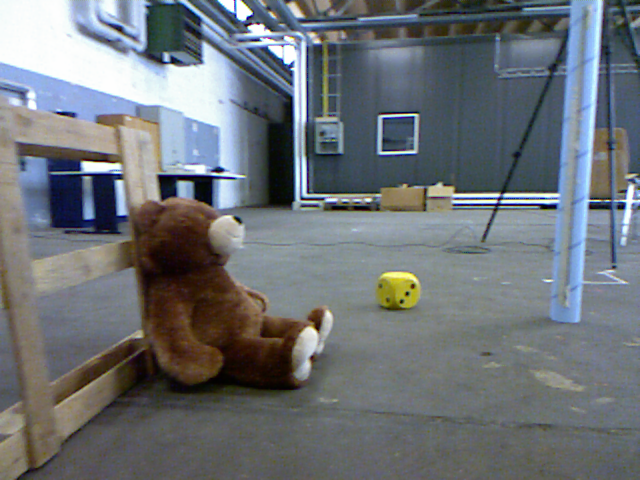
\includegraphics[width=0.30\textwidth]{fr2pioneerslam3}
			}				
			\caption{Sequence samples}
			\label{fig:fig17}
		\end{figure}
	\end{center}
}		

\section{Distance matrix}
\frame{\frametitle{Freiburg 2 Pioneer Slam}
	\begin{center}
		\begin{figure}[ht]
			\subfloat[Distance matrix - M2DP]{%
				\includegraphics[width=0.45\textwidth]{distances_fr2_pioneer_slam_m2dp}
			}
			~
			\subfloat[Distance matrix - CM2DP (ours)]{%
				\includegraphics[width=0.45\textwidth]{distances_fr2_pioneer_slam_cm2dp}
			}			
			\label{fig:fig18}
		\end{figure}
	\end{center}
}

\section{Stereo Matching}
\frame{\frametitle{Stereo Matching}
	\begin{center}
		\begin{figure}[ht]
			\subfloat{%
				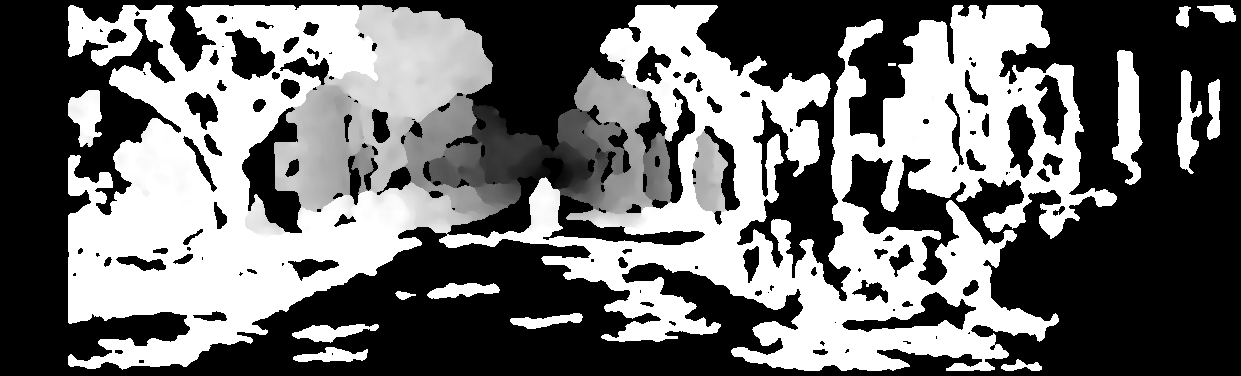
\includegraphics[width=0.50\textwidth]{kitti001}
			}
			~						
			\subfloat{%
				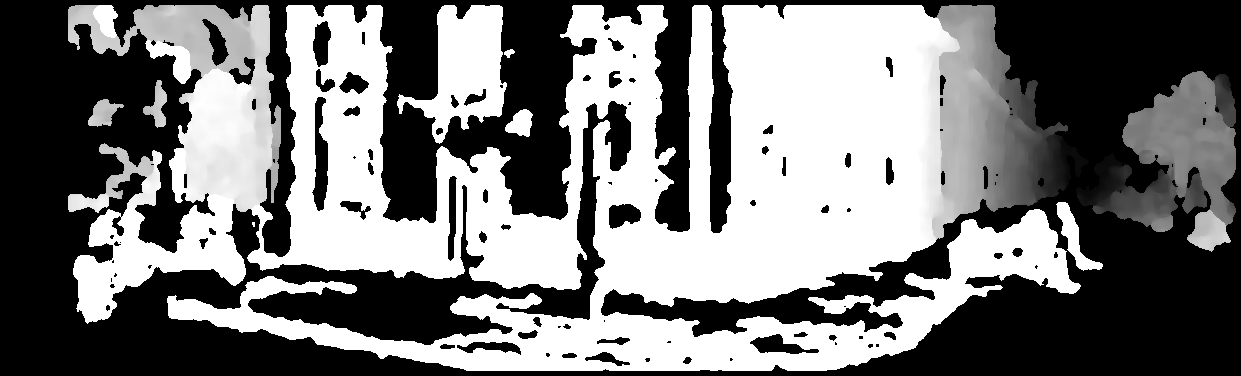
\includegraphics[width=0.50\textwidth]{kitti002}
			}
			
			\subfloat{%
				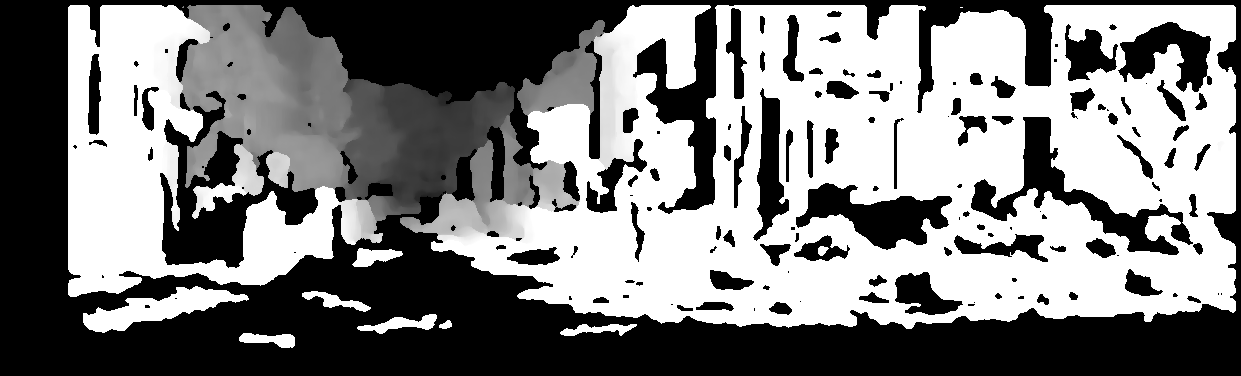
\includegraphics[width=0.50\textwidth]{kitti003}
			}
			~
			\subfloat{%
				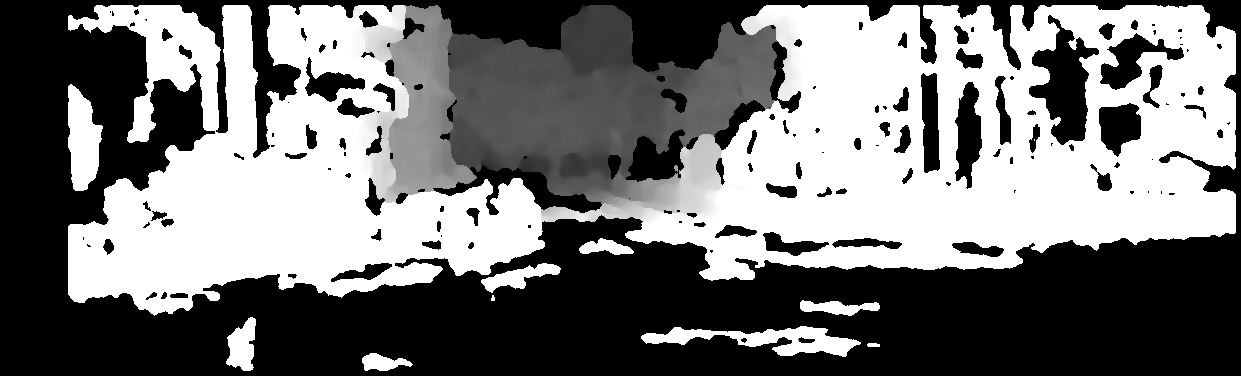
\includegraphics[width=0.50\textwidth]{kitti004}
			}				
			\caption{KITTI 00 - Stereo matching}
			\label{fig:fig19}
		\end{figure}
	\end{center}
}

\section{Result}
\frame{\frametitle{Result}
	\begin{center}
		\begin{figure}[ht]
			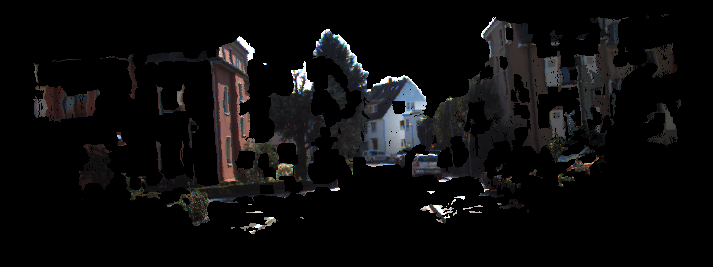
\includegraphics[width=\textwidth]{kitticloud}
			\caption{KITTI 00 - Sample cloud}
			\label{fig:fig20}
		\end{figure}
	\end{center}
}
	
\nocite{*}

\end{document}




